\begin{frame}
  \insertsection{}
  \begin{itemize}
    \item \cite{sabbah_cimpa90} §2.2.2 Asymptotic expansions
    \item \cite{van2003galois} Chap. 7 Exact Asymptotics
  \end{itemize}
  and
  \begin{itemize}
    \item \cite{majima1984asymptotic}
    \item \cite{zbMATH00060600}
    \item \cite{wasow2002asymptotic}
  \end{itemize}
\end{frame}

\begin{frame}
  Let \textcolor{red!60!black}{$U$} be an open interval in $S^1$
  \begin{itemize}
    \item $\Delta_r^*(U):=
      \{z\in\Delta_r\mid z=\rho e^{i\theta},0<\rho<r,\theta\in U\}$%
\footnote{$\Delta_r:=\Delta_r^*(S^1)$}
  \end{itemize}
  \begin{center}
    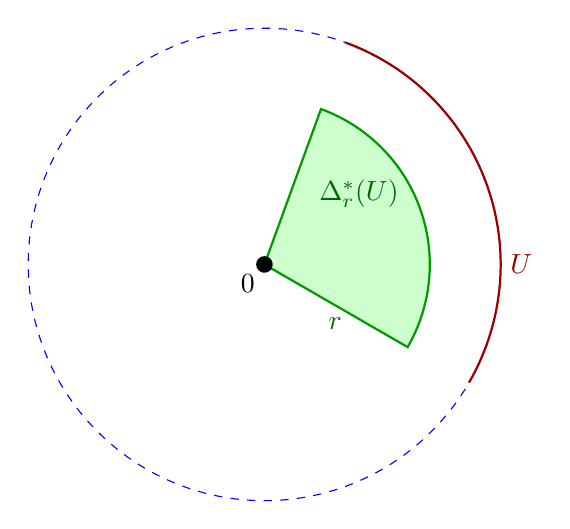
\begin{tikzpicture}[scale=3]
      \node (zero) at (0,0) {};
      \node[below left] at (zero) {$0$};
      \draw[blue,dashed] (zero) circle (1cm);

      \filldraw[fill=green!20!white,draw=green!60!black,thick] (0,0)
        -- ({cos( -30 )*.7},{sin( -30 )*.7}) arc (-30:70:.7) -- cycle;
      \node[green!40!black] at (.4,.3) {$\Delta_r^*(U)$};
      \node[green!40!black] at (.3,-.25) {$r$};

      \draw[thick,red!60!black] ({cos( -30 )},{sin( -30 )}) arc (-30:70:1);

      \node[red!60!black,right] at (1,0) {$U$};

      \fill (zero) circle (1pt);
    \end{tikzpicture}
  \end{center}
\end{frame}

\begin{frame}{Asymptotic expansion}
Let $\hat\phi=\sum_{n\geq -n_0}a_nx^n$ with $a_n\in\C$ is as asymptotic
expansion of $f$ at $0$ if for all $m\in\N$ one has
\begin{equation} \label{eq:asymptoticExpansion}
  \lim_{x\to 0,x\in\triangle_r^*(U)}
  \left|x^{-m}\right|\left|x^{n_{0}}f(x)-\sum_{0\leq n\leq m}a_{n}x^{n}\right|
  =0
\end{equation}
Define
\begin{itemize}
  \item $\bar\cA(U,r)\subset\cO(\Delta_r^*(U))$ the set of functions which
    admits an asymptotic power series
  \item $\cA(U,r):=\bigcap_{V}\bar\cA(V,r)$ where $V$ are relatively
    compact open subsets of $U$
    \begin{itemize}
      \item $\cA(U,r)=\{\phi\in \bar\cA(U,r)
        \mid \phi\in \bar\cA(V,r)
        \forall V\text{ rel.\  cp.\  op.\  subset of }U\}$
    \end{itemize}
  \item $\cA(U):=\bigcup_r\cA(U,r)$%
    \begin{itemize}
      \item $\cA(U)=\{\phi\mid\exists r\text{: } \phi\in\cA(U,r)\}
        =\{\phi\mid\exists r\text{: }
          \forall V\subset U\text{ rel.cp.op.}\text{: }
          \phi\in\bar\cA(V,r)\}$
    \end{itemize}
\end{itemize}
The mapping $U\mapsto\cA(U)$ defines a sheaf on $S^1$
\end{frame}

\begin{frame}
  The equation (\ref{eq:asymptoticExpansion}) says:
  \newcommand{\myto}{\textcolor{gray!60!black}{\overset{x\to0}{\xrightarrow{x\in\triangle_r^*(U)}}}}
  \begin{align*}
    m&=0&
    \left|a_{0}-x^{n_{0}}f(x)\right| &\myto 0
  \\ m&=1&
    \left|a_{0}\frac{1}{\left|x\right|}+a_{1}\frac{x}{\left|x\right|}
    -\frac{x^{n_{0}}f(x)}{\left|x\right|} \right|&\myto 0
  \\ m&=2&
    \left|a_{0}\frac{1}{\left|x^{2}\right|}+a_{1}\frac{x}{\left|x^2\right|}
    +a_{2}\frac{x^2}{\left|x^2\right|}
    -\frac{x^{n_{0}}f(x)}{\left|x^{2}\right|}\right| &\myto 0
  \\ m&=3&
    \left|a_{0}\frac{1}{\left|x^{3}\right|}
    +a_{1}\frac{x}{\left|x^{3}\right|}
    +a_{2}\frac{x^2}{\left|x^3\right|}
    +a_{3}\frac{x^3}{\left|x^3\right|}
    -\frac{x^{n_{0}}f(x)}{\left|x^{3}\right|} \right|&\myto 0
  \\&&&\qquad\vdots
  \\ &&
    \left|a_{0}\frac{1}{\left|x^{m}\right|}
    +a_{1}\frac{x}{\left|x^{m}\right|}+\dots
    +a_{m-1}\frac{x^{m-1}}{\left|x^m\right|}
    +a_{m}\frac{x^{m}}{\left|x^m\right|}
    -\frac{x^{n_{0}}f(x)}{\left|x^{m}\right|} \right|&\myto 0
  \\&&&\qquad\vdots
  \end{align*}
  \begin{exmp}
    \begin{enumerate}
      \item $f=\frac{1}{x}$ \Rightarrow{} $\hat f=x$
        \textcolor{red}{\lightning}
    \end{enumerate}
  \end{exmp}
\end{frame}

\begin{frame}{Other deffinitions}
  \begin{itemize}
    \item \cite[2]{majima1984asymptotic} says:
      $f\in\cA(U)$ iff for every \textbf{closed} subsector and for every
      $N\in\N$
      \[
        \sup_{x\in\bar\cA(V,\tilde r)}
          \left|x^{-N}\left(f(x)-\sum_{i=0}^{N-1}a_ix^i\right)\right|
        <+\infty
      \]
    \item \cite{zbMATH00060600} defines:
      \textbf{asymptotic expansion of Grevrey order $s$}
    \item \cite{wasow2002asymptotic} defines:
      Let the function $f(x)$ be defined in a point-set $S$ of the complex
      $x$-plane having $x=0$ as an accumulation point. The power series
      $\sum_{r=0}^\infty a_rx^r$ is said to represent $f(x)$ asymptotically, as
      $x\to0$ is $S$, if
      \[
        x^{-m}\left[f(x)-\sum_{r=0}^ma_rx^r\right]
      \]
      tends to zero, for all $m\geq0$, as $x$ tends to zero in $S$.
  \end{itemize}
\end{frame}

\begin{frame}{Some elementary properties (2.2.4)}
  \begin{enumerate}
    \item If $\hat\phi$ is an Asymptotic expansion for $f$ then one has
      \[
        a_0=\lim_{x\to 0,x\in\Delta_r^*(U)}x^{n_0}f(x)
      \]
      and for $m>0$,
      \[
        a_m=\lim_{x\to 0,x\in\Delta_r^*(U)}x^{-m}
          \left[x^{n_0}f(x)-\sum_{0\leq n\leq m-1}a_nx^n\right]
      \]
      In particular this asymptotic expansion is unique
      \begin{itemize}
        \item $f$ admits a zero asymptotic expansion iff for all $p\in\Z$
          one has
          \[
            \lim_{x\to 0,x\in\Delta_r^*(U)}x^pf(x)=0
          \]
      \end{itemize}
    \item
      Define $\cA(U)\to \hat K$ denoted by $f\mapsto \hat{f}$.
      \begin{itemize}
        \item $\cA(U)$ is a subring of $\cO(\Delta_r^*(U))$
        \item this mapping is a morphism of rings
      \end{itemize}
    \item Denote by $\cA^{<0}(U)$ the kernel of this morphism
      \begin{itemize}
        \item $x\mapsto e^{-\frac{1}{x}}$ has zero asymptotic expansion in
          some sector around $\theta=0$
      \end{itemize}
    \item $\cA(U)$ is stable under derivation\footnote{Proof in
      \cite{sabbah_cimpa90}}.
    \item $\cA(U)$ contains $K$ as a subfield.
  \end{enumerate}
\end{frame}

\begin{frame}{Borel-Ritt lemma}
  \begin{lem}[2.2.5]
  If $U$ is a proper open interval of the unit circle the mapping
  \[
  \cA(U)\to\hat{K}
  \]
  is onto\footnote{1p proof at \cite{sabbah_cimpa90}[p63]}.
  \end{lem}

  It follows from this lemma that one has an exact sequence
  \[
    0 \to \cA^{<0}(U) \to \cA(U) \to \hat{K} \to 0 \,.
  \]
\end{frame}

\begin{frame}{Main result}
  \begin{thm}[2.3.1]
    Let $\cM_K$ be a meromorphic connection. There exists an integer $q\geq 1$
    such that, after the ramification $x=t^q$, one has, for all $\theta\in S^1$
    and each sufficiently small interval $V$ centered at $\theta$
    \[
      \cA_L(V)\otimes_L\cM_L \cong
        \cA_L(V)\otimes_L\left(\cF_L^R\otimes\cG_L\right)
    \]
  \end{thm}
\end{frame}
